\chapter{Simulations of halo response}
\label{chap:sims-hals}

This chapter briefly describes the methods employed in studying halo relaxation through simulations. Currently, the most accurate description of the relaxation response of a halo to galaxy formation is provided by the hydrodynamical simulations of cosmological volumes that include comprehensive baryonic prescription for a variety of unresolved astrophysical processes.

\section{Hydrodynamical simulations with galaxies}
\label{sec:sims}
Here we describe the cosmological simulations employed in this work; these are from three different publicly available suites namely IllustrisTNG, EAGLE and CAMELS simulations.
\subsection{IllustrisTNG}
\label{sec:sims-IllTNG}
The IllustrisTNG simulations, conducted by the TNG collaboration, employed the \textsc{arepo} code \citep[][]{2020ApJS..248...32W}, which utilizes a moving mesh approach defined by Voronoi tessellation \citep[][]{2010MNRAS.401..791S}. These simulations incorporate an updated model of galaxy formation that includes cosmic magnetic fields in addition to major baryonic processes such as cooling, star formation, and stellar and AGN feedback \citep[][]{2017MNRAS.465.3291W,2018MNRAS.473.4077P}. The suite comprises three cosmological boxes: TNG50, TNG100, and TNG300, with periodic box sizes of $35 \Mpch$, $75 \Mpch$, and $200 \Mpch$, respectively, consistent with the cosmology from \cite{2016A&A...594A..13P}. Initial conditions were generated at $z=127$ using the Zel'dovich approximation \citep[][]{1970A&A.....5...84Z} with the \textsc{N-GenIC} code \citep[][]{2015ascl.soft02003S}. 

We utilize the highest resolution runs from all three boxes to study a wide range of halo responses to galaxy formation. Specifically, TNG50 offers sufficient resolution for low-mass haloes, while TNG300 provides an adequate number of cluster-scale haloes. Throughout our analysis, we utilize data from redshifts $z=0$ to $z=5$ from IllustrisTNG for both hydrodynamical and corresponding gravity-only runs. This allows us to examine the effects of baryonic processes on dark matter halo properties across different scales and epochs.

\subsection{EAGLE}
\label{sec:sims-EAGLE}
The EAGLE (Evolution and Assembly of GaLaxies and their Environments) cosmological simulations were conducted using a modified version of the \textsc{gadget-3} code, which employs smoothed particle hydrodynamics \citep[][]{2005MNRAS.364.1105S}. Initial conditions were generated using the \textsc{ic\_2lpt\_gen} code following \cite{2010MNRAS.403.1859J}. The main large-volume simulation was performed in a cosmological volume of $(100 ~\rm{Mpc})^3$ periodic box with its reference model of galaxy formation, incorporating sub-grid prescriptions for various baryonic processes such as cooling, star formation, and feedback mechanisms \citep[][]{2015MNRAS.446..521S,2015MNRAS.450.1937C}. This reference model of EAGLE simulations has been shown to produce realistic galaxies \citep[][]{2015MNRAS.448.2941S,2015MNRAS.450.4486F,2015MNRAS.452.2879T}. 

In addition, this suite includes multiple small-volume simulations with wide variations in the baryonic subgrid prescriptions for astrophysical processes. These simulations were performed at the same resolution as the large-volume reference simulation but in a $25 ~\rm{Mpc}$ periodic box. The variations include adjustments to the gas equation of state, the threshold for star formation, efficiency of stellar feedback, the viscosity of the black-hole accretion disk and the nature of stochastic heating caused by AGN feedback. In particular we study these following simulations:

\begin{itemize}
    \item \textbf{Ref} (Reference model): This simulation uses the standard EAGLE subgrid physics parameters but in this smaller box.
    \item \textbf{eos53} : This considers a gas equation of state $\gamma = 5/3$.
    \item \textbf{eos1} : This considers an isothermal gas equation of state $\gamma = 1$.
    \item \textbf{FixedSfThresh}: This uses a constant threshold for star formation independent of the metallicity.
    \item \textbf{WeakFB}: This follows a lower efficiency of stellar feedback that is scaled down by $50 \%$ compared to the reference simulation.
    \item \textbf{StrongFB}: This follows a higher efficiency of stellar feedback, twice that of the reference simulation.
    \item \textbf{NoAGN}: AGN feedback is disabled in this simulation to study the effects of stellar feedback alone.
    \item \textbf{AGNdT8}: In this, the temperature of gas raised by the AGN feedback heating is  lower with $\Delta T_{\rm{AGN}} = 10^8$K from the reference value of $\Delta T_{\rm{AGN}} = 10^{8.5}$K.
    \item \textbf{AGNdT9}: In this, the temperature of gas raised by the AGN feedback heating is higher with $\Delta T_{\rm{AGN}} = 10^9$K from the reference value of $\Delta T_{\rm{AGN}} = 10^{8.5}$K.
    \item \textbf{RefHR}: This simulation uses the same EAGLE subgrid prescription as `Ref' simulation but at a $8 times$ higher mass resolution.
    \item \textbf{RecalHR}: This simulation uses the same resolution as `RefHR' but with recalibrated EAGLE subgrid prescription.
\end{itemize}
We use the redshift $z=0$ data from this set of simulations along with their corresponding gravity-only run to study the role of different astrophysical processes on the relaxation response of the halo.



\subsection{CAMELS}
\label{sec:sims-CAMELS}
The Cosmology and Astrophysics with MachinE Learning Simulations (CAMELS) project comprises a comprehensive suite of hydrodynamical simulations designed to explore the interplay between cosmological and astrophysical parameters in shaping the universe's large-scale structure \cite[][]{CAMELS_presentation}. These simulations are performed in a relatively smaller cosmological volume of $(25 \ \mathrm{Mpc}/h)^3$, containing $256^3$ dark matter particles and an equivalent number of baryonic particles \cite{CAMELS_DR1}.

In our study, we specifically utilize the TNG suite's 1P set of simulations, a subset that methodically varies one parameter at a time to isolate the effects of individual parameters in the TNG model. For our analysis, we concentrate on parameters related to supernova (SN) feedback and active galactic nucleus (AGN) feedback, each governed by the following two distinct parameters:
% 
\begin{itemize}
    \item \textbf{Supernova Feedback Parameters:}
    \begin{itemize}
        \item $A_{\mathrm{SN1}}$: Varied between 0.25 to 4, this parameter controls the energy flux of the galactic winds. It is implemented as a prefactor for the overall energy output per unit star formation rate \cite{2018MNRAS.473.4077P,CAMELS_presentation}.
        \item $A_{\mathrm{SN2}}$: Varied between 0.5 to 2, this parameter controls the speed of the galactic winds. For a fixed $A_{\mathrm{SN1}}$, changes in $A_{\mathrm{SN2}}$ affect the galactic wind speed in concert with the mass-loading factor to maintain a fixed energy output.
    \end{itemize}
    \item \textbf{AGN Feedback Parameters:}
    \begin{itemize}
        \item $A_{\mathrm{AGN1}}$: Varied between 0.25 to 4, this parameter controls the overall power injected in the kinetic feedback mode of AGN. It is implemented as a prefactor for the energy per unit black-hole accretion rate \cite{2017MNRAS.465.3291W,CAMELS_presentation}.
        \item $A_{\mathrm{AGN2}}$: Varied between 0.5 to 2, this parameter controls the burstiness and the temperature of the heated gas during AGN feedback "bursts" by changing the wind speed of the AGN feedback.
    \end{itemize}
\end{itemize}
% 
All these parameters have a value of one in the fiducial simulation, and there are five simulations with higher values and another five simulations with lower values for each of these parameters. In total, we utilize these 41 hydrodynamical simulations and compare them against the gravity-only simulation over the same cosmological volume.



\subsection{Halo matching}
\label{sec:methods-match-ch:z0main}
To study how a dark halo responded to the galaxy forming in it, we need to first reliably match the catalogue of haloes found in the hydrodynamic simulation (which includes galaxy formation physics) to those found in its gravity-only run. For various numerical reasons a given halo in the hydro run may not have a true match in the halo catalogue of gravity-only run. So we first try to obtain an exhaustive catalogue of matched haloes that will be used to build a statistical description of this halo response.


\subsubsection{Matching procedure}
We match the haloes using the particle data associated with the haloes;
while the mass of each dark matter particle differs between the hydrodynamical and gravity-only runs, the \emph{number} of dark matter particles within the same initial periodic box is the same for each of the five pairs of simulations that we consider in IllustrisTNG and EAGLE. So a given particle in a hydro simulation has originated from the same region as the particle of the same ID in its corresponding gravity-only run.
For any given pair of haloes, with one in the hydrodynamical simulation and the other in the corresponding gravity-only run, we define the matching fraction of each of those two haloes (with respect to the other) 
as the fraction of its dark matter particles that are also present in the other halo. Below, we describe how we use 
these matching fractions to decide if the given pair can be considered a valid matched pair. 


\begin{figure}
    \centering
    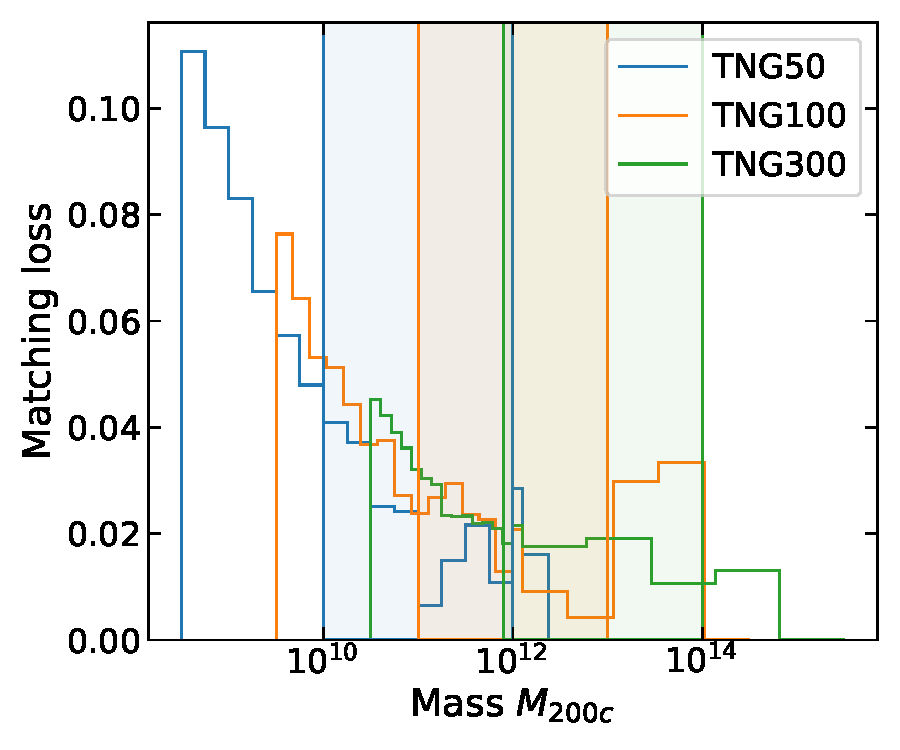
\includegraphics[width=\linewidth]{plots/hal_match_efficiency_mass_all.pdf}
    \caption{Fraction of haloes in the TNG hydrodynamical simulations that have not found a match is shown as a function of mass $M_{200c}$. coloured vertical bands represent the mass range relevant for this work in each of the three TNG simulation boxes.}
    \label{fig:matching-loss-all-ch:z0main}
\end{figure}

\begin{figure}
\centering
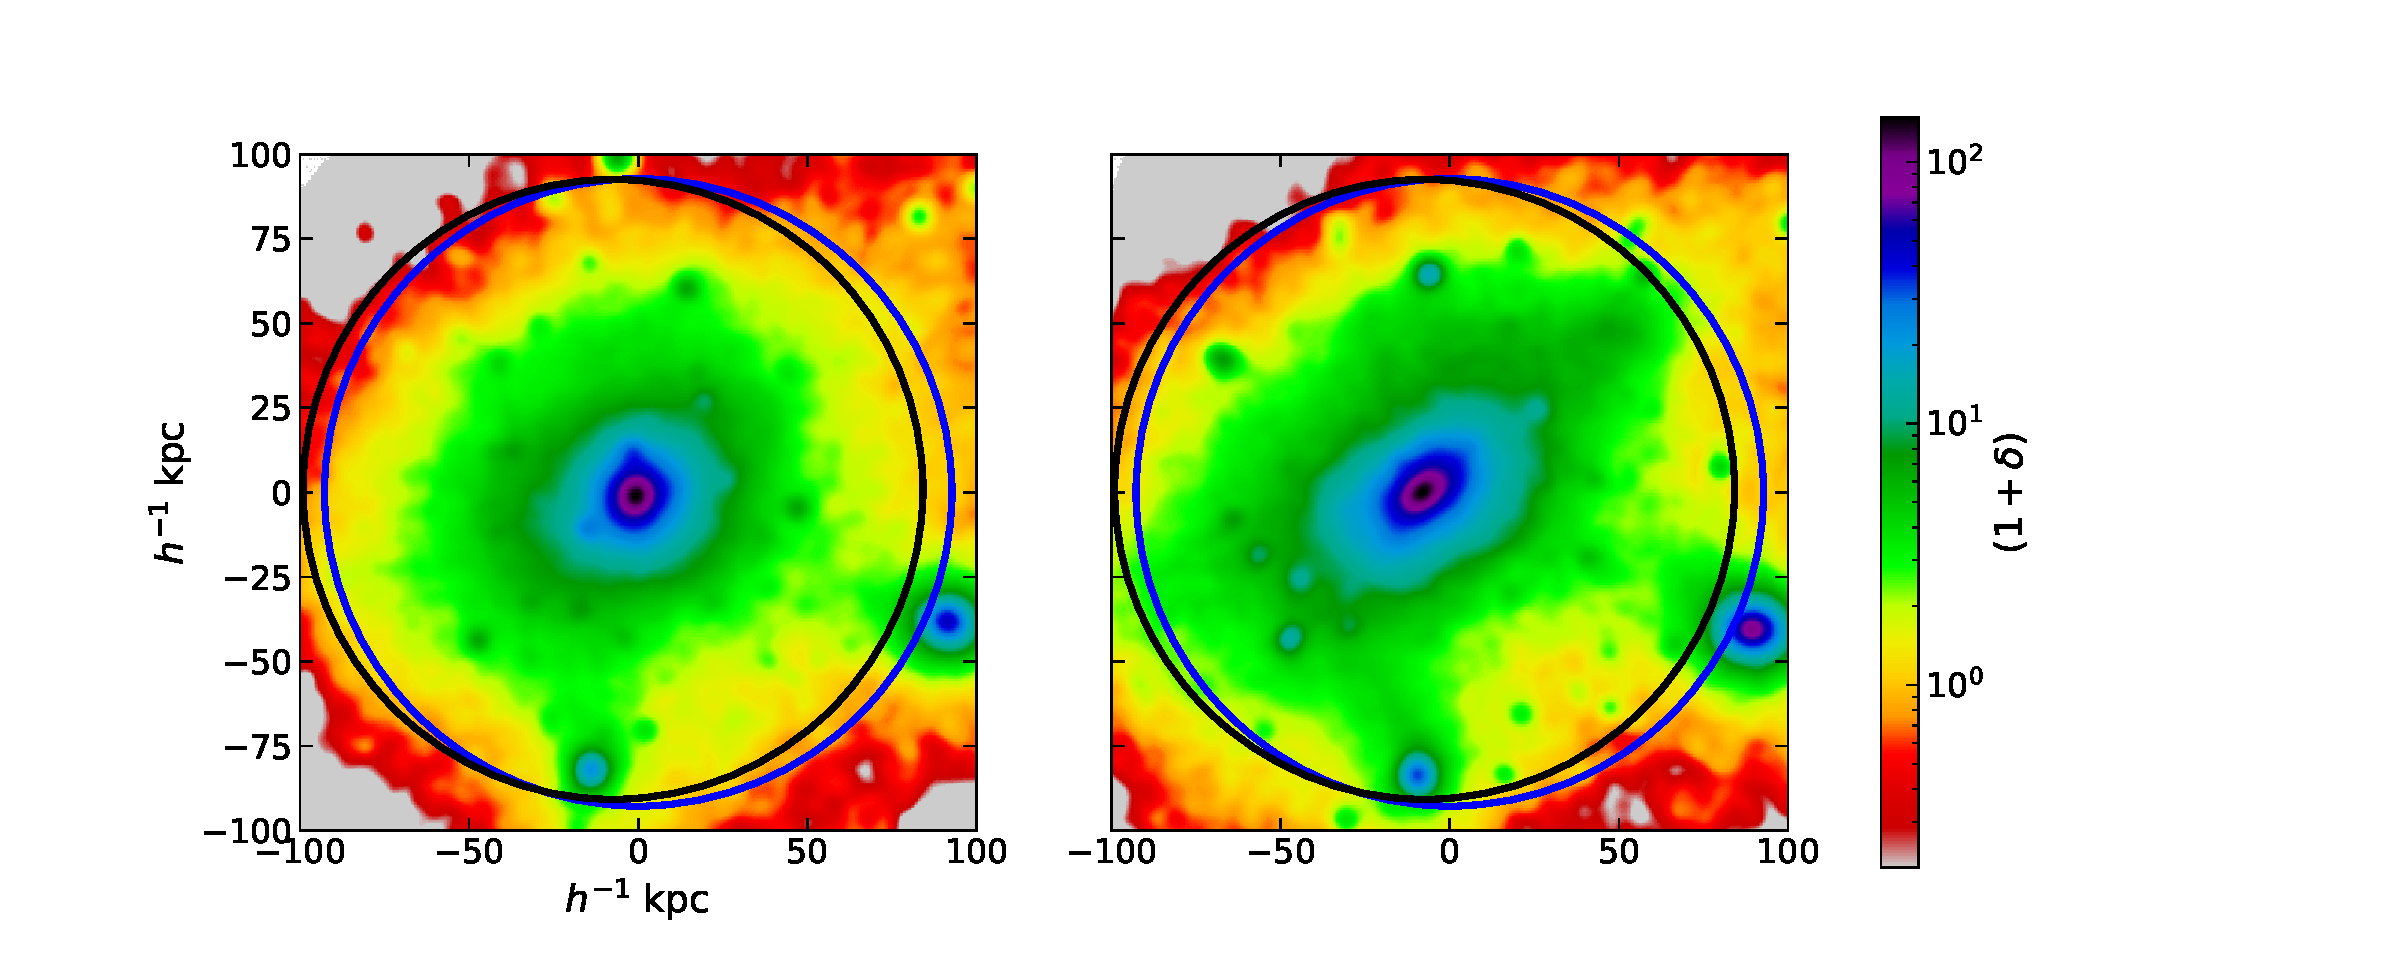
\includegraphics[clip,trim={0.5cm 0cm 2cm 0.5cm}, width=\linewidth]{plots/visual_single_halo.pdf}
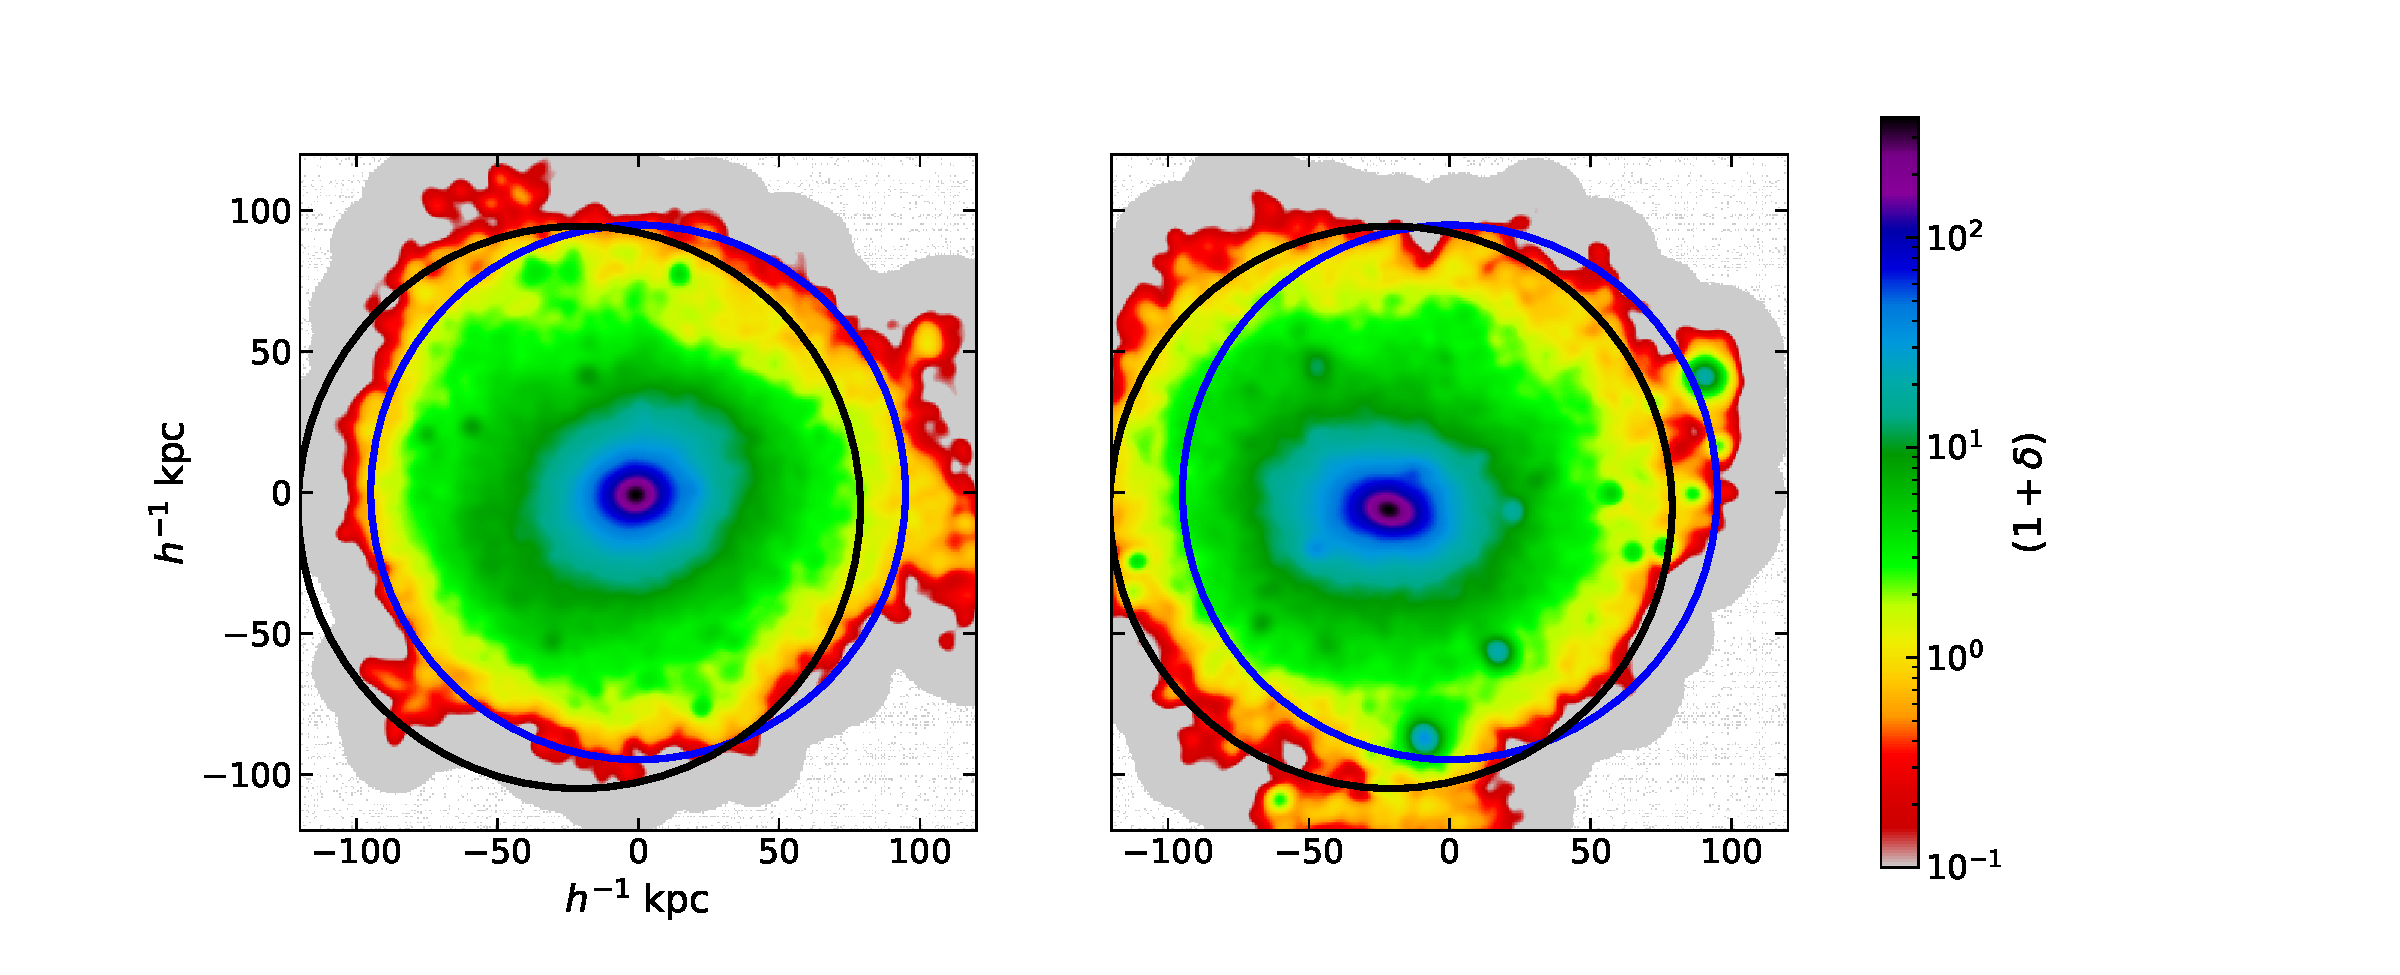
\includegraphics[clip,trim={0.5cm 0cm 2cm 0.5cm}, width=\linewidth]{plots/visual_single_halo_E.pdf}
\caption{Visually inspecting two matched FOF halo pairs, one each from IllustrisTNG \emph{(top row)} and EAGLE \emph{(bottom row)} using 2D-projected dark matter density field around the center of the hydrodynamical halo in a thick slice. The \emph{left panel} shows the halo in the hydrodynamical simulation and the \emph{right panel} shows the corresponding matched pair in the gravity-only simulation. The black circle shows the virial boundary of the gravity-only halo and blue circle shows that of the hydrodynamical halo. In both cases, the hydrodynamical halo is noticeably more spherical and compact than its gravity-only counterpart, with a spatially offset center. See text for a discussion.} 
\label{fig:single-halo-pair-ch:z0main}
\end{figure}

Computing the matching fractions 
for every pair of haloes is computationally expensive with $O(n^2)$ for millions of haloes in the catalogue. We decrease the complexity to $O(n)$ by supplying, for each halo in the hydro-simulation, an ordered list of most probable match candidates in the gravity-only run. These candidate lists of gravity-only haloes are generated and ranked based on the spatial positions of the haloes and their masses using a KD-tree based neighbour finding algorithm, implemented using \texttt{scipy.spatial.KDTree}.
For each halo in the hydro run, we test if the matching fraction of this halo with respect to any of the haloes in its match candidate list exceeds the value of 0.5. This ensures that at most one halo is selected as a match for each of the hydrodynamical haloes, so that our matched catalogue of halo pairs will be a subset of the source catalogue without repetitions.
While we match as many haloes as possible, it is also important to ensure that false matches don't plague our study. Based on the results in Appendix \ref{sec:apndx-matching-ch:z0main}, we therefore additionally require that in a valid matched pair, the gravity-only FOF halo must also have a matching fraction of more than 0.5 with respect to the hydrodynamical halo.
Our FOF based matching can be compared with
\citet[][]{2018MNRAS.481.1950L} where a similar matching algorithm has been followed for central subhaloes.

\subsubsection{Halo pair catalogue}
We generate a matched catalogue of haloes for each of the five simulations studied in this work, including FOF haloes resolved with more than 1000 particles\footnote{Mass resolution in the gravity-only runs are $7 \times 10^7 \Mh$, $8.9 \times 10^6 \Mh$ and $5.4 \times 10^5$ for TNG300, TNG100 and TNG50 respectively; whereas $9.7 \times 10^6 \Mh$ for the L100 and $1.21 \times 10^6 \Mh$ for the L25 simulation of EAGLE.}. The fraction of hydrodynamical haloes that fails to be part of the matched catalogue is shown in \figref{fig:matching-loss-all-ch:z0main} in bins of halo mass for the IllustrisTNG simulations. %
In the mass range in which the halo samples are selected for this work (see \secref{sec:results-mass-ch:z0main}), more than 96\% of the haloes in hydrodynamical simulation have been assigned a match in the gravity-only run. The small fraction of unmatched haloes primarily reside in dense environments 
where our algorithm presumably fails due to
the inherent issues with 3D FOF algorithm in dealing with mergers. Similar results hold for the EAGLE simulations as well. 
For illustrative purpose, a visual representation of two randomly chosen halo pairs, one each from IllustrisTNG and EAGLE, is shown in \figref{fig:single-halo-pair-ch:z0main}. 










\subsection{Methods to study the halo response}
\label{sec:method-ch:z0main}
The response of dark matter halo to galaxy formation has primarily two aspects, contraction or expansion of the halo towards the centre and a change in its triaxial shape. In this work, we study the former aspect of the halo response, by focusing on spherically averaged mass profiles. 
The illustrative haloes shown in \figref{fig:single-halo-pair-ch:z0main} become more compact and spherical in the hydrodynamical simulation that includes galaxy formation.
Also notice that there is an offset between the center-of-potential locations of matched pairs of haloes. These offsets are likely correlated with the halo tidal environment and will be interesting to follow-up in future work.

\subsubsection{Mass profiles}
\label{subsec:massprofiles-ch:z0main}

The overall expansion and/or contraction of dark matter in response to galaxy formation can be studied through the differences in spherically averaged mass profiles between matched haloes. For the dark matter, these radial profiles are obtained by adding up the mass of all dark matter particles contained within concentric spherical shells. In addition to these, we also need baryon mass profiles in modelling the dark matter response. While stellar mass profiles are computed in a similar fashion as dark matter,
for the gas mass profiles we use a Gaussian kernel to assign mass enclosed to each of the spherical shells\footnote{Throughout this work, we consider concentric shells defined by their radii and the mass enclosed by such a shell is the mass in the sphere bounded by that shell.
}. 
The width of this Gaussian kernel was taken to match the SPH smoothing length for the EAGLE simulation, whereas for IllustrisTNG we use the cube root of the Voronoi cell volume to define the kernel smoothing scale. We have tested that our results are robust to differences in the choice of this kernel.


\subsubsection{Quasi-adiabatic relaxation model}
\label{sec:methods-adiab-ch:z0main}
The impact of galaxy formation on the dark halo is expected to be primarily an adiabatic relaxation of dark matter particle orbits in response to baryon condensation \citep[][]{1986ApJ...301...27B}. We start by discussing this simplified model and study more complex effects such as the impact of baryonic feedback processes below.
Assuming that the dark matter halo is spherical and doesn't undergo shell crossing while baryons condense towards the centre, the adiabatic relaxation of any given dark matter shell is determined by the change in baryonic mass within that shell. 
Consider a shell enclosing a \emph{dark matter} mass $M_i^d(r_i)$ in radius $r_i$ in the unrelaxed halo. After relaxation, the radius of the shell changes to $r_f$. By definition, the dark matter mass $M_f^d(r_f)$ enclosed in $r_f$ in the relaxed halo is simply
\be 
M_f^d(r_f) = M_i^d(r_i)\,.
\label{eq:DMmass1-ch:z0main}
\ee
The \emph{total} mass $M_i(r_i)$ enclosed in $r_i$ in the unrelaxed halo, on the other hand, does not necessarily equal the total mass $M_f(r_f)$ enclosed in $r_f$ in the relaxed halo.
If angular momentum were to be conserved and the dark matter particle orbits stay circular, then the amount of relaxation of the shell is completely determined by the change in this total mass within the shell
\citep[][]{1986ApJ...301...27B},
\begin{align}
    r_i \,M_i(r_i) = r_f \,M_f(r_f) %
    \implies 
\frac{r_f}{r_i} = \frac{M_i(r_i)}{M_f(r_f)}\,. 
\label{eq:AR1-ch:z0main}
\end{align}
Extending this idealised scenario, quasi-adiabatic relaxation models consider the relaxation ratio $r_f/r_i$ as a function of the mass ratio $M_i/M_f$.
\begin{align}
\frac{r_f}{r_i} &= 1 + \chi \left( \frac{M_i(r_i)}{M_f(r_f)} \right) 
\label{eq:qAR1-ch:z0main}
\end{align}
For example, the baryonification procedures in \cite{2015JCAP...12..049S,2021MNRAS.503.4147P} include dark matter response as a quasi-adiabatic relaxation with
\be
\chi(y) = q\,(y-1)\,.
\label{eq:chi-linear-ch:z0main}
\ee

\subsubsection{The relaxation relation} %
\label{sec:methods-relx-reln-ch:z0main}
Our focus in this work is to characterise the relaxation relation \eqn{eq:qAR1-ch:z0main} as a function of halo and galaxy properties over a wide dynamic range; e.g, we would like to ask whether \eqn{eq:chi-linear-ch:z0main} is a good description of this relation.
To study this, we must extract this relation for individual haloes in hydrodynamical simulations.
For a given hydrodynamical halo in the matched catalog, we can obtain this relaxation relation by considering its matched halo in the gravity-only run to represent its unrelaxed state. 
We find it convenient to work with $r_f$ as a control variable. In this case, the values of $r_i$, $M_i(r_i)$ and $M_f(r_f)$ must be obtained from the matched halo pair, which can be done as follows.

For a dark matter shell at radius $r_f$ in the relaxed halo enclosing a dark matter mass of $M_f^d(r_f)$, its unrelaxed radius $r_i$ can be obtained by applying \eqn{eq:DMmass1-ch:z0main} and inverting the mass profile $M_i^d(r)=(1-f_b) M_i(r)$ of the gravity-only halo, where $f_b$ is the cosmic baryon fraction, to obtain 
\begin{align}
\label{eq:inv-mass-ch:z0main}
r_i = {M_i}^{-1} \left( \frac{M_f^d(r_f)}{(1-f_b)} \right)\,.
\end{align}
This is because each `particle' in the gravity-only halo consists of collisionless baryons and dark matter in precisely the proportion $f_{b}$. 
The value of $M_i(r_i)$ then follows from direct mass counting in the unrelaxed (i.e., gravity-only) halo in radius $r_i$, and the value of $M_f(r_f)$ follows from direct mass counting in the relaxed (i.e. hydrodynamical) halo in radius $r_f$, as described in \secref{subsec:massprofiles-ch:z0main}. In practice, we first obtain the unrelaxed mass profile $M_i(r_i)$ for a wide range of radii in finely spaced bins, in order to then compute the inverse in \eqn{eq:inv-mass-ch:z0main} by interpolation.

Thus, for any shell defined by its relaxed radius $r_f$, we can obtain both the relaxation ratio $r_f/r_i$ and the mass ratio $M_i/M_f$ from its unrelaxed radius computed from mass profiles. Hence we can obtain the relaxation relation by placing multiple concentric shells around the halo all the way to its virial radius $R_{\rm{vir}}$.
In Appendix \ref{appen:Mock-ch:z0main}, we have tested this algorithm on mock halo + galaxy systems generated with fixed known relaxation relations.


% \section{Techniques}
% \label{sec:methods}
\section{Haloes with relaxation}
In the simulations from IllustrisTNG and EAGLE suites, 3D friend-of-friends (FoF) algorithm \citep[see][for details]{2016A&C....15...72M,2019ComAC...6....2N} was used to obtain halo group catalogues. And the \textsc{subfind} code \citep{2001MNRAS.328..726S} was used to identify the subhaloes within these FoF group haloes as gravitationally bound substructures. Within each FoF group halo, the subhalo enclosing the gravitational potential minimum is assigned as its central subhalo. This trough in the gravitational potential is used to define the centre of that halo. Its size is characterized by the `virial' radius $R_{\rm vir}\equiv R_{\rm 200c}$ defined as the radius of the sphere around its centre enclosing a mean matter density that is 200 times the cosmological critical density. Its mass is then defined as the corresponding total mass enclosed $M\equiv M_{200c}$. In the simulations from the CAMELS suite, the haloes were identified in the  phase-space by a 6D FoF algorithm using the \textsc{rockstar} code. We characterize sizes and masses using the same quantities  $R_{\rm 200c}$ and $M_{\rm 200c}$ respectively.
% is defined as the `virial' radius $R_{\rm vir}\equiv R_{\rm 200c}$ of a given FoF group halo; while the total mass enclosed within this radius quantifies the mass of the halo $M\equiv M_{200c}$.

% Following our previous work \citep{2023Velmani&Paranjape}, 
To study the relaxation response of dark matter, we match the haloes from the full hydrodynamic simulations with the haloes in the corresponding gravity-only runs performed over same cosmological volumes. We identify these matched halo pairs based on the amount of overlap in their proto halo patches. In particular, this involves identifying nearby haloes of similar sizes between the hydrodynamical and gravity-only simulations and then match them by simulation particles \cite{2023Velmani&Paranjape}.
%  From this catalogue, we select populations of matched halo pairs by the logarithmic mass of the gravity-only halo $(\log(M/\Mh))$ in bins centred at $11.5, 12, 12.5, 13, 13.5, 14$ with a bin width of 0.3 at redshift $z=0.01$. While the small volume TNG50 offers well-resolved low-mass haloes $10^{11.5} \Mh$ and $10^{12} \Mh$, the TNG100 cosmological box gives $10^{12.5} \Mh$ and $10^{13} \Mh$ haloes and the largest volume TNG300 provides an adequate number of cluster-scale haloes of masses $10^{13.5} \Mh$ and $10^{14} \Mh$. 


\section{Relaxation Response Modeling}
\label{sec:methods-relmodel}
In the catalogues of matched halo pairs, hydrodynamical ones with galaxies are considered relaxed, while the gravity-only counterparts represent unrelaxed dark haloes. The relaxation response of dark matter within a halo, is generally evaluated through variations in their radial mass profiles indicating contraction or expansion due to the galaxy.  These spherically averaged dark matter profiles are computed by the cumulative sum of the mass contributed by all dark matter particles within concentric spherical shells. For the gravity-only halo, the cosmic dark matter fraction of the mass in each particle is considered as contributing to the dark matter. 

We employ the quasi-adiabatic relaxation framework to characterize the relaxation from these profiles.
% \subsection{Quasi-adiabatic relaxation}
% \label{sec:methods-adiab}
The relaxation response in cold dark matter occurs entirely due to gravitational interactions with baryons. This is an aggregate effect of the baryonic mass flow resulting from galactic processes such as inflows and feedback. The quasi-adiabatic relaxation model is a physically motivated framework that relates the change in the spherically averaged dark matter distribution at a given time to the spherically averaged baryonic distribution at the same time. This baryonic profile encompasses all non-dark matter mass, including gas and stars.

Earlier models assumed spherical halo where the dark matter particles maintain their radial ordering while responding adiabatically to baryonic particle flows \citep[][]{1986ApJ...301...27B}. In this scenario, if a dark matter particle initially at radius \( r_i \) in the unrelaxed halo moves to radius \( r_f \) in the relaxed halo, the enclosed dark matter mass within these radii remains equal.
\begin{equation} 
M_f^d(r_f) = M_i^d(r_i)\,.
\label{eq:DMmass}
\end{equation}

However, due to the baryonic mass flow, the total mass enclosed within these spheres is not necessarily equal, \( M_i(r_i) \neq M_f(r_f) \). Further assumption of angular momentum conservation for dark matter particles in circular orbits, implies that the change in total enclosed mass must be consistent with the amount of relaxation \citep[][]{1986ApJ...301...27B}.
\begin{align}
    r_i \,M_i(r_i) = r_f \,M_f(r_f) %
    \implies 
    \frac{r_f}{r_i} = \frac{M_i(r_i)}{M_f(r_f)}\,. 
\label{eq:AR}
\end{align}
% 
The \textbf{Quasi-adiabatic relaxation framework} empirically extends this idealized scenario by considering the relaxation ratio \( r_f/r_i \) as a function of the mass ratio \( M_i/M_f \).
\begin{align}
\frac{r_f}{r_i} &= 1 + \chi \left( \frac{M_i(r_i)}{M_f(r_f)} \right) 
\label{eq:qAR}
\end{align}
In a straightforward extension, the baryonification procedures described in \cite{2015JCAP...12..049S,2021MNRAS.503.4147P} incorporate dark matter response as a quasi-adiabatic relaxation with 
\be
\chi(y) = q\,(y-1)\,.
\label{eq:chi-linear}
\ee
Various quasi-adiabatic models have been proposed, offering different approaches to this framework \citep{2010MNRAS.407..435A,2004ApJ...616...16G,2023Velmani&Paranjape}.


\section{Haloes}

\section{Characterizing the halo response}